% $Header: /cvsroot/latex-beamer/latex-beamer/solutions/conference-talks/conference-ornate-20min.en.tex,v 1.6 2004/10/07 20:53:08 tantau Exp $

\documentclass[trans]{beamer}
\usepackage{etex}
\newcommand\orh{\mbox{ ; }}
% This file is a solution template for:

% - Talk at a conference/colloquium.
% - Talk length is about 20min.
% - Style is ornate.



% Copyright 2004 by Till Tantau <tantau@users.sourceforge.net>.
%
% In principle, this file can be redistributed and/or modified under
% the terms of the GNU Public License, version 2.
%
% However, this file is supposed to be a template to be modified
% for your own needs. For this reason, if you use this file as a
% template and not specifically distribute it as part of a another
% package/program, I grant the extra permission to freely copy and
% modify this file as you see fit and even to delete this copyright
% notice.
%\usepackage{xcolor}
\usepackage{graphicx}
\usepackage{array}
\usepackage[all]{xy}
%\usepackage{theapa}
\usepackage{tikz}
\usetikzlibrary{shapes.geometric}
\usetikzlibrary{shadows}
\usetikzlibrary{positioning}
\usepackage{algorithm}
%\usepackage{algorithmic}
\usepackage{algpseudocode}
\usepackage{natbib}
\usepackage{apalike}
\mode<presentation>
{
%  \usetheme{AnnArbor}
%  \usetheme{Antibes}
%  \usetheme{Bergen}
%  \usetheme{Berkeley}
%  \usetheme{Berlin}
%  \usetheme{Boadilla}
%  \usetheme{boxes}
%  \usetheme{CambridgeUS}
%  \usetheme{Copenhagen}
%  \usetheme{Darmstadt}
%  \usetheme{default}
%  \usetheme{Dresden}
%  \usetheme{Frankfurt}
%  \usetheme{Goettingen}
%  \usetheme{Hannover}
%  \usetheme{Ilmenau}
%  \usetheme{JuanLesPins}
%  \usetheme{Luebeck}
%  \usetheme{Madrid}
%  \usetheme{Malmoe}
%  \usetheme{Marburg}
%  \usetheme{Montpellier}
%  \usetheme{PaloAlto}
%  \usetheme{Pittsburgh}
%  \usetheme{Rochester}
%  \usetheme{Singapore}
%  \usetheme{Szeged}
%  \usetheme{Warsaw}
  \usetheme{PLP}

%\usecolortheme{lily}%
  % or ...

  \setbeamercovered{transparent}
  % or whatever (possibly just delete it)
}


\usepackage[english]{babel}
% or whatever

%\usepackage[latin1]{inputenc}
% or whatever

\usepackage{times}
\usepackage[T1]{fontenc}
% Or whatever. Note that the encoding and the font should match. If T1
% does not look nice, try deleting the line with the fontenc.
\newcommand{\myalert}[1]{{%\color{red}
 #1}}
\newcommand{\fluffy}{\mathit{fluffy}}
\newcommand{\bdd}[2]
{
\begin{center}
\begin{tikzpicture}
[every node/.style={font=\scriptsize,minimum height=0.5cm,minimum width=0.5cm},x=2cm,y=1.2cm,rounded corners=2mm,zeroarrow/.style = {-stealth,dashed},
  onearrow/.style = {-stealth,solid},
  c/.style = {circle,draw,solid,minimum width=2em,
        minimum height=2em},
  r/.style = {rectangle,draw,solid,minimum width=2em,
        minimum height=2em}]
%[place/.style={shape=ellipse}]
%,draw=blue!50,fill=blue!20,thick,inner sep=0pt,minimum size=6mm},

\node[c] (X11) at (0,1) {#1};
   \node[c] (X21) at (1,1.5) {#2};
   \node[r] (final-one) at (2,0.5) {1};
   \node[r] (final-zero) at (2,1.5){0};
\node[] (lX11) at (0,0) {#1};
   \node (lX21) at (1,0) {#2};


   \path[onearrow,bend right=20] (X11) edge (final-one) ;
   \path[onearrow,bend right=20] (X21) edge   (final-one) ;

%      \draw[onearrow] (X11) -- (final-one);
%   \draw[onearrow] (X21) -- (final-one);

   \path[zeroarrow,bend left=20] (X11) edge  (X21) ;
   \path[zeroarrow,bend left=20] (X21) edge  (final-zero) ;
%
%   \draw[zeroarrow] (X11) -- (X21);
%   \draw[zeroarrow] (X21) -- (final-zero);
%
%\node (root) at ( 0,1) {};
%\node (node21) at ( 1,1.5){}  ;
%\node (0) at ( 2,1.5) {0};
%\node (1) at ( 2,0.5) {1};
%\path[-,bend left](node21) edge (0) (root) edge node {0} (node21);
%\path[-,bend right]
%			 (root) edge (1)
%(node21) edge (1);
\end{tikzpicture}
\end{center}
}


\newcommand{\mdd}
{
\begin{center}
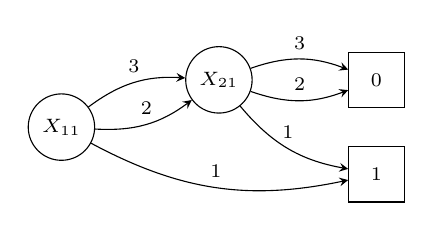
\begin{tikzpicture}
[every node/.style={font=\scriptsize},x=2cm,y=1.2cm,
zeroarrow/.style = {-stealth,dashed},
  onearrow/.style = {-stealth,solid},
  c/.style = {circle,draw,solid,minimum width=2em,
        minimum height=2em},
  r/.style = {rectangle,draw,solid,minimum width=2em,
        minimum height=2em}]
%[place/.style={shape=ellipse}]
%,draw=blue!50,fill=blue!20,thick,inner sep=0pt,minimum size=6mm},

\node[c] (X11) at (0,1) {$X_{11}$};
   \node[c] (X21) at (1,1.5) {$X_{21}$};
   \node[r] (final-one) at (2,0.5) {1};
   \node[r] (final-zero) at (2,1.5){0};

   \path[onearrow,bend right=20] (X11) edge   node [above,midway] {1}(final-one) ;
   \path[onearrow,bend right=20] (X21) edge   node [above,midway] {1}(final-one) ;

   \path[onearrow,bend right=20] (X11) edge   node [above,midway] {2}(X21) ;
   \path[onearrow,bend left=20] (X11) edge   node [above,midway] {3}(X21) ;
   \path[onearrow,bend right=20] (X21) edge   node [above,midway] {2}(final-zero) ;
   \path[onearrow,bend left=20] (X21) edge   node [above,midway] {3}(final-zero) ;
%
%\node (root) at ( 0,1) {};
%\node (node21) at ( 1,1.5){}  ;
%\node (0) at ( 2,1.5) {0};
%\node (1) at ( 2,0.5) {1};
%\path[-,bend left](node21) edge (0) (root) edge node {0} (node21);
%\path[-,bend right]
%			 (root) edge (1)
%(node21) edge (1);
\end{tikzpicture}
\end{center}
}
\newcommand{\mn}{
\begin{center}
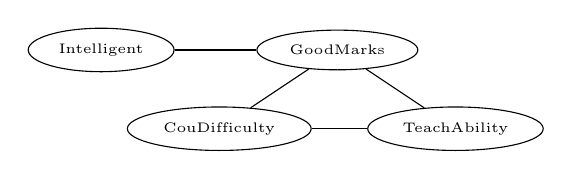
\begin{tikzpicture}
[every node/.style={ellipse,draw,font=\tiny},x=1.5cm,y=1cm]
%[place/.style={shape=ellipse}]
%,draw=blue!50,fill=blue!20,thick,inner sep=0pt,minimum size=6mm},
\node (VisitToAsia) at ( 0,1) {Intelligent};
\node (Tubercolosis) at ( 2,1) [ellipse,draw] {GoodMarks};
\node (Asthma) at ( 1,0) [ellipse,draw] {CouDifficulty};
\node (Cough) at ( 3,0) [ellipse,draw] {TeachAbility};
\path (VisitToAsia) edge  (Tubercolosis)
			 (Tubercolosis) edge (Asthma) edge (Cough)
			(Asthma) edge (Cough);
\end{tikzpicture}\end{center}}

\newcommand{\mln}{
\begin{center}
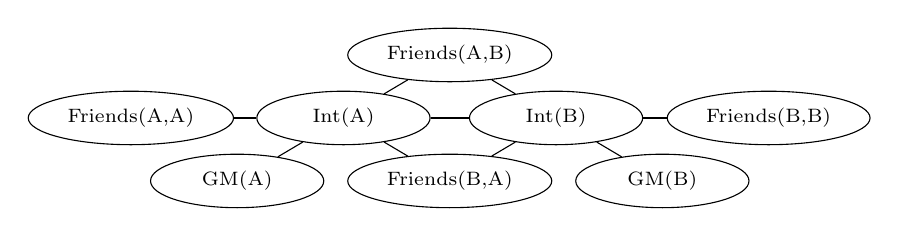
\begin{tikzpicture}
%[every node/.style={ellipse,draw,font=\scriptsize,minimum height=0.5cm,minimum width=2.5cm,
[every node/.style={ellipse,draw,font=\scriptsize,minimum width=2.2cm},x=2.7cm,y=0.8cm]

%[place/.style={shape=ellipse}]
%,draw=blue!50,fill=blue!20,thick,inner sep=0pt,minimum size=6mm},
\node (FriendsAB) at ( 1.5,2) {Friends(A,B)};
\node (FriendsAA) at ( 0,1)  {Friends(A,A)};
\node (FriendsBB) at ( 3,1)  {Friends(B,B)};
\node (FriendsBA) at ( 1.5,0)  {Friends(B,A)};
\node (SmokesA) at ( 1,1)  {Int(A)};
\node (SmokesB) at ( 2,1)  {Int(B)};
\node (CancerA) at ( 0.5,0)  {GM(A)};
\node (CancerB) at ( 2.5,0)  {GM(B)};
\path (FriendsAA) edge  (SmokesA)
		(CancerA) edge (SmokesA)
	(FriendsBB) edge  (SmokesB)
		(CancerB) edge (SmokesB)
	(FriendsAB) edge  (SmokesA)
					edge  (SmokesB)
	(FriendsBA) edge  (SmokesA)
					edge  (SmokesB)
			(SmokesB) edge (SmokesA);

%			 (Tubercolosis) edge (Asthma) edge (Cough)
%			(Asthma) edge (Cough);
\end{tikzpicture}
\end{center}
}


\newcommand{\bn}{
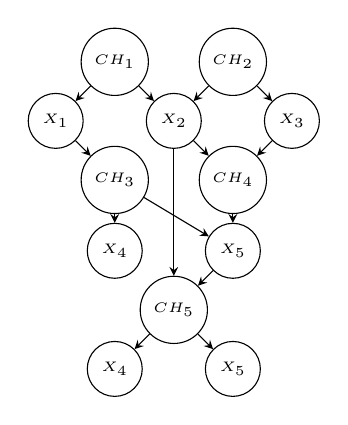
\begin{tikzpicture}
[every node/.style={draw,font=\tiny},x=0.75cm,y=0.75cm,rounded corners=2mm,zeroarrow/.style = {-stealth,dashed},
  onearrow/.style = {-stealth,solid},
  c/.style = {circle,draw,solid},
  r/.style = {rectangle,draw,solid,minimum width=1em,
        minimum height=1em}]
%[place/.style={shape=ellipse}]
%,draw=blue!50,fill=blue!20,thick,inner sep=0pt,minimum size=6mm},

\node[c] (CH1) at (1,5) {$CH_1$};
\node[c] (CH2) at (3,5) {$CH_2$};
\node[c] (X1) at (0,4) {$X_1$};
\node[c] (X2) at (2,4) {$X_2$};
\node[c] (X3) at (4,4) {$X_3$};
\node[c] (CH3) at (1,3) {$CH_3$};
\node[c] (CH4) at (3,3) {$CH_4$};
\node[c] (X4) at (1,1.8) {$X_4$};
\node[c] (X5) at (3,1.8) {$X_5$};
\node[c] (CH5) at (2,0.8) {$CH_5$};
\node[c] (X6) at (1,-0.2) {$X_4$};
\node[c] (X7) at (3,-0.2) {$X_5$};
%
%   \node[c] (X21) at (1,1.5) {#2};
%   \node[r] (final-one) at (2,0.5) {1};
%   \node[r] (final-zero) at (2,1.5){0};
%
%
   \path[onearrow] (CH1) edge (X1) ;
   \path[onearrow] (CH1) edge (X2) ;
   \path[onearrow] (CH2) edge (X2) ;
   \path[onearrow] (CH2) edge (X3) ;
   \path[onearrow] (X1) edge (CH3) ;
   \path[onearrow] (X2) edge (CH4) ;
   \path[onearrow] (X3) edge (CH4) ;
   \path[onearrow] (CH3) edge (X4) ;
   \path[onearrow] (CH3) edge (X5) ;
   \path[onearrow] (CH4) edge (X5) ;
   \path[onearrow] (X2) edge (CH5) ;
   \path[onearrow] (X5) edge (CH5) ;
   \path[onearrow] (CH5) edge (X6) ;
   \path[onearrow] (CH5) edge (X7) ;

%
%%      \draw[onearrow] (X11) -- (final-one);
%%   \draw[onearrow] (X21) -- (final-one);
%
%   \path[zeroarrow,bend left=20] (X11) edge  (X21) ;
%   \path[zeroarrow,bend left=20] (X21) edge  (final-zero) ;
%
%   \draw[zeroarrow] (X11) -- (X21);
%   \draw[zeroarrow] (X21) -- (final-zero);
%
%\node (root) at ( 0,1) {};
%\node (node21) at ( 1,1.5){}  ;
%\node (0) at ( 2,1.5) {0};
%\node (1) at ( 2,0.5) {1};
%\path[-,bend left](node21) edge (0) (root) edge node {0} (node21);
%\path[-,bend right]
%			 (root) edge (1)
%(node21) edge (1);
\end{tikzpicture}
}
%\addtobeamertemplate{background canvas}{\transuncover}{}

\title[PLP - Ch 4]
{Foundations of Probabilistic Logic Programming}
\subtitle{Chapter 4: Semantics for Hybrid Programs}

\author[F. Riguzzi] % (optional, use only with lots of authors)
{Fabrizio Riguzzi}
% - Give the names in the same order as the appear in the paper.
% - Use the \inst{?} command only if the authors have different
%   affiliation.

\institute[] % (optional, but mostly needed)
{
%ENDIF -- University of Ferrara,  Italy\\
% fabrizio.riguzzi@unife.it
}
% - Use the \inst command only if there are several affiliations.
% - Keep it simple, no one is interested in your street address.


\subject{cplint}
% This is only inserted into the PDF information catalog. Can be left
% out.



% If you have a file called "university-logo-filename.xxx", where xxx
% is a graphic format that can be processed by latex or pdflatex,
% resp., then you can add a logo as follows:

\date{}


% Delete this, if you do not want the table of contents to pop up at


% If you wish to uncover everything in a step-wise fashion, uncomment
% the following command:

%\beamerdefaultoverlayspecification{<+->}
%\AtBeginSection[]
%{
%\begin{frame}
%\frametitle{Outline}
%\end{frame}
%}
\begin{document}
\begin{frame}
\titlepage
\vspace{-2cm}
\begin{center}
\includegraphics[scale=0.120]{plp-book.jpg}

\includegraphics[scale=0.3]{cc-by.png}

\end{center}
\end{frame}



\begin{frame}
  \frametitle{Hybrid Programs}
\begin{itemize}
\item Up to now only discrete random variables and discrete probability distributions. 
\item Hybrid Probabilistic Logic Programs: some of the random variables are continuous.
\item cplint allows the specification of density functions over arguments of atoms in the head of rules
\end{itemize}
\end{frame}

\begin{frame}[fragile]
  \frametitle{Hybrid Programs}
\begin{itemize}
\item A probability density on an argument \verb|Var| of an atom \verb|A| is specified with
\begin{verbatim}
A : Density :- Body.
\end{verbatim}
where \verb|Density| is a special atom 
\begin{itemize}
\item 
\verb|uniform(Var,L,U)|: \verb|Var|  is uniformly distributed in $[L,U]$
\item 
\verb|gaussian(Var,Mean,Variance)|:  Gaussian distribution 
\item 
\verb|dirichlet(Var,Par)|:  Dirichlet distribution with parameters $\alpha$ specified by the list \verb|Par|
\item 
\verb|gamma(Var,Shape,Scale)|: gamma distribution 
\item 
\verb|beta(Var,Alpha,Beta)|:  beta distribution 
\item + others (see the manual)
\end{itemize}
\end{itemize}
\end{frame}

\begin{frame}[fragile]
  \frametitle{Hybrid Programs}
  \begin{itemize}
\item 
Also discrete distribution, with either a finite or countably infinite support:
\begin{itemize}
\item 
\verb|discrete(Var,D)| or \verb|finite(Var,D)|:  \verb|D| is a list of couples \verb|Value:Prob| assigning probability \verb|Prob| to \verb|Value|
\item 
\verb|uniform(Var,D)|: \verb|D|  is a list of values each taking the same probability (1 over the length of \verb|D|).
\item 
\verb|poisson(Var,Lambda)|: Poisson distribution 
\end{itemize}
\end{itemize}
\end{frame}

\begin{frame}[fragile]
  \frametitle{Examples}
  \begin{center}
\begin{verbatim}
g(X) : gaussian(X,0,1).
\end{verbatim}
\includegraphics[width=0.27\textwidth]{normal.pdf}
\begin{verbatim}
g(X) : gaussian(X,[0,0],[ [1,0],[0,1] ]).
\end{verbatim}
\includegraphics[width=0.3\textwidth]{2dgauss.pdf}
\end{center}
\end{frame}

\begin{frame}[fragile]
  \frametitle{Inference}
  \begin{itemize}
\item If an atom encodes a continuous random variable (such as \verb|g(X)| above), asking the probability that a ground instantiation, such as \verb|g(0.3)|, is true is not meaningful, as the probability that a continuous random variables takes a specific value is always 0.
\item In this case you are more interested in computing the distribution of \verb|X| of a goal \verb|g(X)|, possibly after having observed some evidence.
\end{itemize}
\end{frame}
\begin{frame}[fragile]
  \frametitle{Gaussian Mixture Example}
  \begin{itemize}
  \item
 \url{http://cplint.eu/e/gaussian_mixture.pl} defines a mixture of two Gaussians:
\begin{verbatim}
heads:0.6;tails:0.4.
g(X): gaussian(X,0, 1).
h(X): gaussian(X,5, 2).
mix(X) :- heads, g(X).
mix(X) :- tails, h(X).
\end{verbatim}
\item
The argument \verb|X| of
\verb|mix(X)| follows a distribution that is a mixture of two Gaussian,
one with mean 0 and variance 1 with probability 0.6 and one with 
mean 5 and variance 2 with probability 0.4.
\end{itemize}
\end{frame}
\begin{frame}[fragile]
  \frametitle{Gaussian Mixture Example}
  \begin{itemize}
\item We can  perform the query
\begin{verbatim}
mc_sample_arg(mix(X),1000,X,Values).
\end{verbatim}
\item \verb|histogram/3| draws a histogram of values
\begin{verbatim}
histogram(+List:list,-Chart:dict,+Options:list).
\end{verbatim}
\item possible \verb|Options|:
\begin{itemize}
\item \verb|min(+Min:float)| the minimum value of domain, default value the minimum in List
\item \verb|max(+Max:float)| the maximum value of domain, default value the maximum in List
\item \verb|nbins(+NBins:int)| the number of bins for dividing the domain, default value 40
\end{itemize}
\end{itemize}
\end{frame}
\begin{frame}[fragile]
  \frametitle{Gaussian Mixture Example}
  \begin{itemize}
\item Probability density function of \verb|X|, we can use
\begin{verbatim}
mc_sample_arg(mix(X),1000,X,_Values), 
  histogram(_Values,Chart,[]).
\end{verbatim}

\end{itemize}
\end{frame}
\begin{frame}[fragile]
  \frametitle{Posterior estimation in Bayesian models Example}
  \begin{itemize}
  \item
The parameters of the distribution atoms can be taken from the probabilistic
atom, the example \url{http://cplint.eu/e/gauss_mean_est.pl}
\begin{verbatim}
val(I,X) :-
  mean(M),
  val(I,M,X).
mean(M): gaussian(M,1.0, 5.0).
val(_,M,X): gaussian(X,M, 2.0).
\end{verbatim}
  \item
states that for an index \verb|I| the continuous variable \verb|X| is 
sampled from a Gaussian whose variance is 2 and whose mean is sampled from a Gaussian with mean 1 and
variance 5.
\end{itemize}
\end{frame}
\begin{frame}[fragile]
  \frametitle{Kalman Filter Example}
  \begin{itemize}
  \item
Any operation is allowed on continuous random variables.  Kalman filter
\url{http://cplint.eu/e/kalman_filter.pl}:
\begin{tiny}
\begin{verbatim}
kf(N,O, T) :-
  init(S),
  kf_part(0, N, S,O,T).
kf_part(I, N, S,[V|RO], T) :-
  I < N,
  NextI is I+1,
  trans(S,I,NextS),
  emit(NextS,I,V),
  kf_part(NextI, N, NextS,RO, T).
kf_part(N, N, S, [],S).
trans(S,I,NextS) :-
  {NextS =:= E + S},
  trans_err(I,E).
emit(NextS,I,V) :-
  {NextS =:= V+X},
  obs_err(I,X).
init(S):gaussian(S,0,1).
trans_err(_,E):gaussian(E,0,2).
obs_err(_,E):gaussian(E,0,1).
\end{verbatim}
\end{tiny}
\item In case random variables are not sufficiently instantiated to 
exploit expressions for inferring the values of other variables, 
inference will return an error.
\end{itemize}
\end{frame}

\begin{frame}[fragile]
  \frametitle{Conditional Queries}
  \begin{itemize}
\item You can also execute conditional queries over hybrid programs.
\item Sampling arguments of goals representing continuous random variables and drawing a probability density of the sampled argument. 
\item Three cases
  \begin{enumerate}
\item The evidence does not contain atoms with continuous random variables (the probability of evidence is different from 0).
\item The evidence contains atoms with continuous random variables, but its probability is not zero.
\item The evidence contains the grounding of atoms with continuous random variables (its probability is 0).
\end{enumerate}
\item 
For the first two cases you can use the predicates \verb|mc_rejection_sample_arg/6| and \verb|mc_mh_sample_arg/6|.
\end{itemize}
\end{frame}


\begin{frame}[fragile]
  \frametitle{Conditional Queries, Case 1}
  \begin{itemize}
  \item Take 1000 samples of \verb|X| in mix(X) given that heads was true using rejection sampling and Metropolis-Hastings MCMC
\begin{verbatim}
mc_rejection_sample_arg(mix(X),heads,1000,X,_V), 
  histogram(_V,Chart,[]).
mc_mh_sample_arg(mix(X),heads,1000,X,_V,[lag(2)]), 
  histogram(_V,Chart,[]).
\end{verbatim}
  \end{itemize}
\end{frame}
\begin{frame}[fragile]
  \frametitle{Conditional Queries, Case 2}
  \begin{itemize}
  \item Take 1000 samples of \verb|X| in \verb|mix(X)| given that \verb|X>2| was true using rejection sampling and draw an histogram of the probability density of \verb|X|
\begin{verbatim}
mc_rejection_sample_arg(mix(X),(mix(Y),Y>2),
  1000,X,_V,), histogram(_V,Chart,[]).
mc_mh_sample_arg(mix(X),(mix(Y),Y>2),1000,X,
  _Values,[lag(2)]),histogram(_Values,Chart,[]).
\end{verbatim}
  \end{itemize}
\end{frame}
\begin{frame}
  \frametitle{Conditional Queries, Case 3}
   \begin{itemize}
  \item  When you have evidence on ground atoms that have continuous values as arguments (probability of the evidence is 0),  you need to use likelihood weighting 
  \item
  For each sample to be taken, likelihood weighting uses a meta-interpreter to find a sample where the goal is true
  \item Then a different meta-interpreter is used to evaluate the evidence attaching a  weight to the sample.
  \item  Each time the meta-interpreter encounters a probabilistic choice over a continuous variable, it it was already  sampled, it computes the probability density of the sampled value and multiplies the weight by it.     \end{itemize}
\end{frame}
\begin{frame}[fragile]
  \frametitle{Posterior estimation in Bayesian models Example}
  \begin{itemize}
\item
Estimating the true value of a Gaussian distributed random variable, given some observed data.
 \item The variance is known (2) and we suppose that the mean has a Gaussian distribution with mean 1 and variance 5.
\item We take different measurement (e.g. at different times), indexed with an integer. Given that we observe 9 and 8 at indexes 1 and 2, how does the distribution of the random variable (value at index 0) changes with respect to the case of no observations?
  \end{itemize}
\end{frame}
\begin{frame}[fragile]
  \frametitle{Posterior estimation in Bayesian models Example}
  \begin{itemize}
\item Likelihood weighing
\begin{verbatim}
mc_lw_sample_arg(:Query:atom,:Evidence:atom,
  +N:int,?Arg:var,-ValList)
\end{verbatim}
\item \verb|ValList| a list of couples \verb|V-W| where \verb|V| is a value of \verb|Arg| for which \verb|Query| succeeds and \verb|W| is the weight computed by likelihood weighting according to \verb|Evidence|
\item Given that we observe 9 and 8 at indexes 1 and 2, what is the distribution of the random variable (value at index 0)?
\begin{verbatim}
mc_lw_sample_arg(val(0,X),(val(1,9),val(2,8)),
  1000,X,V).
\end{verbatim}
  \end{itemize}
\end{frame}
\begin{frame}[fragile]
  \frametitle{Posterior estimation in Bayesian models Example}
   
\begin{verbatim}
density(+List:list,-Chart:dict,+Options:list) 
\end{verbatim}
draws a line chart of the density of the samples in \verb|List| 

   
\begin{verbatim}
densities(+PriorList:list,+PostList:list,-Chart:dict,
  +Options:list)
\end{verbatim}
draws a line chart of the density of two sets of samples, usually prior and post observations. 

 The same options as in \verb|histogram/3|  are recognised.
\begin{scriptsize}
\begin{verbatim}
?-  mc_sample_arg(val(0,X),1000,X,L0,[]),
    histogram(L0,Chart,[]).
?-  mc_sample_arg(val(0,X),1000,X,L0,[]),
    density(L0,Chart,[]).
? - mc_sample_arg(val(0,Y),1000,Y,_V0), 
    mc_lw_sample_arg(val(0,X),(val(1,9),val(2,8)),1000,X,_V),
    densities(_V0,_V,Chart,[]).
\end{verbatim}
\end{scriptsize}
\end{frame}
\begin{frame}[fragile]
  \frametitle{Expectations}
\begin{verbatim}
mc_lw_expectation(:Query:atom,Evidence:atom,
  +N:int,?Arg:var,-Exp:float)
\end{verbatim}
 \begin{itemize}
\item computes the expected value of \verb|Arg| in \verb|Query| given that \verb|Evidence| is true.
\item  It takes \verb|N| samples, weighting each according to the evidence, and returns their weighted average.
\end{itemize}
\end{frame}
\begin{frame}[fragile]
  \frametitle{Particle Filtering}
  \begin{itemize}
\item In some cases  likelihood weighting encounters numerical  problems,
as the weights of samples may go rapidly to very small numbers that can be rounded to
0 by floating point arithmetic. 
\item This happens for example for dynamic models, 
\item \alert{Particle filtering}  periodically resamples the individual samples/particles so that their weight 
is reset to 1.
\item 
In particle filtering, the evidence is a list of literals. A number $n$ of  samples of the query is taken
that are weighted by the likelihood of the first element of the evidence list. 
\item Each sample constitutes a particle and the sampled random variables are stored away. 
\item 
After weighting, $n$ particles are resampled
with replacement with a probability proportional to their weight.
\item Then the next element of the evidence is considered. 
\end{itemize}
\end{frame}
\begin{frame}[fragile]
  \frametitle{Particle Filtering Example}
\url{http://cplint.eu/e/kalman_filter.pl}
\begin{verbatim}
?-[O1,O2,O3,O4]=[-0.133, -1.183, -3.212, -4.586],
  mc_particle_sample_arg([kf_fin(1,T1),kf_fin(2,T2),
  kf_fin(3,T3),kf_fin(4,T4)],
  [kf_o(1,O1),kf_o(2,O2),kf_o(3,O3),kf_o(4,O4)],100,
  [T1,T2,T3,T4],[F1,F2,F3,F4]).
\end{verbatim}
performs particle filtering for a Kalman filter with four observations. For each observation, the value of the state at the same time point is sampled. The list of samples is returned in \verb|[F1,F2,F3,F4]|
\begin{verbatim}
mc_particle_sample(:Query:atom,:Evidence:list,
  +Samples:int,-Prob:float) 
mc_particle_expectation(:Query:atom,Evidence:atom,
  +N:int,?Arg:var,-Exp:float)
\end{verbatim}
\end{frame}
\end{document}
